\chapter{Einleitung}

\begin{quote}
\textbf{Haushaltsaufgaben m�ssen sinnvoll und einfach auf alle Mitbewohner verteilt werden und der aktuelle Stand zu jedem beliebigen Zeitpunkt f�r jeden einsehbar sein.}
\end{quote}
Die App bietet jedem Mitbewohner die M�glichkeit Notizen einzusehen und zu erstellen. Au�erdem ist es M�glich eine Einkaufsliste zu verwalten, in der Artikel hinzugef�gt, gel�scht und als gekauft markiert werden k�nnen. Des Weiteren zeigt ein Putzplan die noch anstehenden bzw. bereits erledigten Aufgaben aus dem WG Haushalt an. Jedes WG-Mitglied kann sich in der App einloggen. Dass ein Smartphone als neues Tr�germedium dient, liegt nahe, weil nahezu alle der durchweg jungen erwachsenen Personen der Zielgruppe solch ein Ger�t besitzen. Au�erdem bietet es mit der hohen Konnektivit�t die perfekte Grundlage alle Mitbewohner jederzeit auf dem gleichen Wissensstand zu halten. Als Betriebssystem kommt die von Google entwickelte Android Plattform zum Einsatz. Durch deren hohen Marktanteil von 68,2\% in Deutschland wird hier die gr��te Anzahl an potentiellen Nutzern erreicht (siehe Abb. \ref{fig:AndroidMarktanteil}).
\clearpage
\begin{figure}[h]
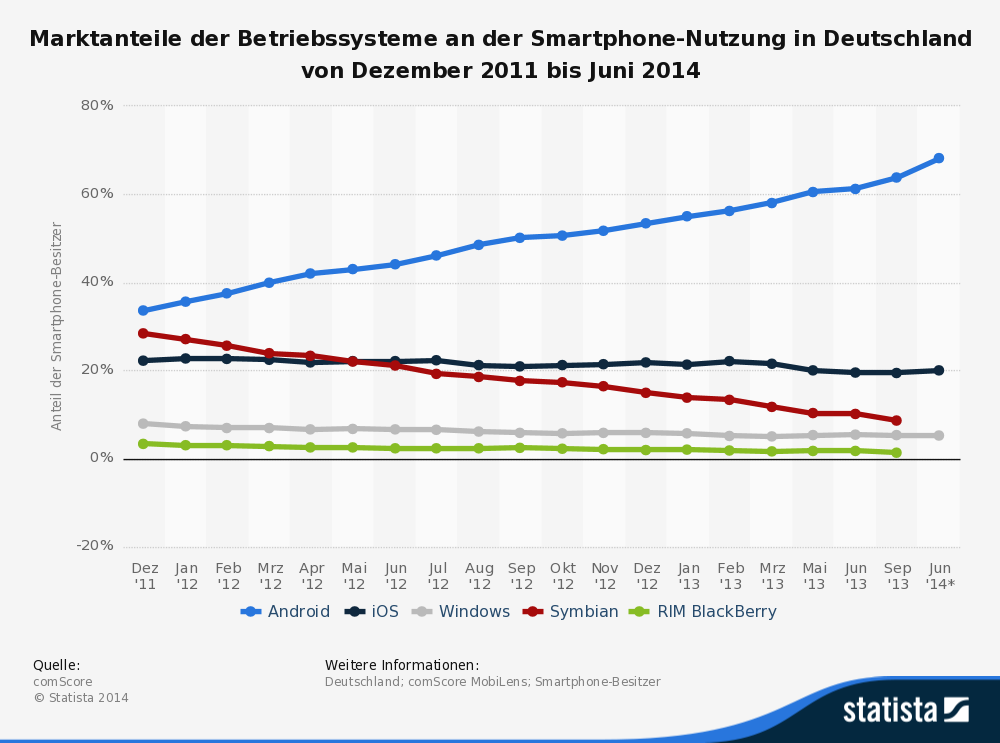
\includegraphics[width=\linewidth]{images/statistic_id170408_marktanteile-der-betriebssysteme-an-der-smartphone-nutzung-in-deutschland-bis-2014}
\caption{Marktanteile der Betriebssysteme an der Smartphone-Nutzung in Deutschland von Dezember 2011 bis Juni 2014}
\label{fig:AndroidMarktanteil}
\end{figure}